\section{Results}\label{sec:results}
% Objective: Model values against disclosed values; the funding-spread inversion; the call attribution; the issuer arithmetic that needs no model.

\subsection{Model value against the disclosed value}

\begin{figure}[tbp]
\centering
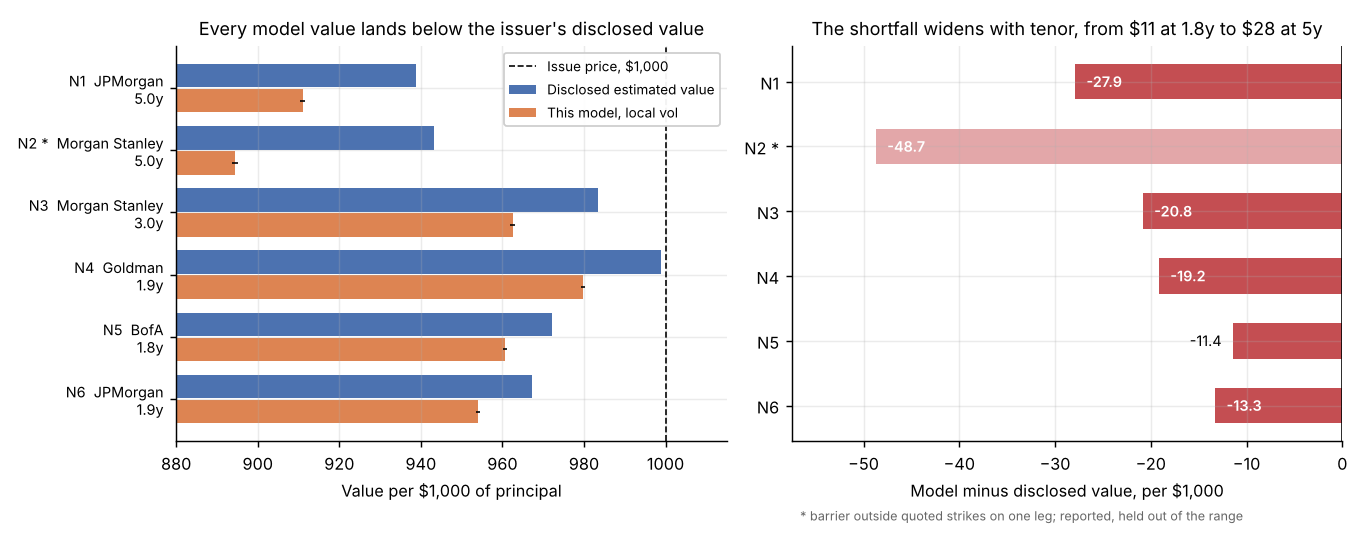
\includegraphics[width=\textwidth]{figures/model_vs_disclosed}
\caption{Model value against the disclosed estimated value, in levels and in
differences, per \$1{,}000 of principal}
\label{fig:gaps}
\notetext{\textit{Notes:} Left panel, the disclosed estimated value and the
model value for each note, with the issue price marked; whiskers are one
standard error of the simulated mean and are smaller than the bar width at this
scale. Right panel, model value less disclosed value. The starred note is
reported but held out of the ranges quoted in the text, for the barrier
coverage reason given in \S\ref{sec:data}. Source:
\texttt{scripts/make\_figures.py}.}
\end{figure}

% Generated by scripts/make_paper_tables.py from the frozen results.
% Do not edit by hand; the next build overwrites it.
\begin{table}[tbp]
\centering
\caption{Model value against the disclosed estimated value, per \$1,000 of principal}
\label{tab:results}
\small
\begin{tabular}{l r r r r r}
\toprule
Note & Model value & s.e. & Disclosed & Gap & Gap (\%) \\
\midrule
N1 & 910.98 & 0.34 & 938.90 & $-$27.92 & $-$2.97 \\
N2\textsuperscript{a} & 894.38 & 0.37 & 943.10 & $-$48.72 & $-$5.17 \\
N3 & 962.56 & 0.29 & 983.40 & $-$20.84 & $-$2.12 \\
N4 & 979.84 & 0.24 & 999.00 & $-$19.16 & $-$1.92 \\
N5 & 960.69 & 0.26 & 972.10 & $-$11.41 & $-$1.17 \\
N6 & 954.01 & 0.30 & 967.30 & $-$13.29 & $-$1.37 \\
\bottomrule
\end{tabular}
\notetext{\textit{Notes:} Model value is the mean discounted payoff over 200,000 paths with a European control variate, at a zero funding spread over the Treasury curve, with the issuer's call exercised by the Longstaff--Schwartz rule. The standard error is of that mean. Gap is model value less disclosed value, so a negative gap means the independent valuation lands below the figure the issuer discloses. Every note shows one. \textsuperscript{a}\,Excluded from the ranges quoted in the text; see Table~\ref{tab:terms}.}
\end{table}


Table~\ref{tab:results} gives the result the rest of the paper is about. Every
model value lands below the issuer's disclosed estimated value. Across the five
notes whose barriers are covered by quoted strikes the shortfall runs from
\$11.41 to \$27.92 per \$1{,}000 of principal, or 1.17 to 2.97 per cent of the
disclosed figure; the note held out of that range is further below still, at
\$48.72. Standard errors are between \$0.24 and \$0.37, so the differences are
one to two orders of magnitude larger than the simulation noise around them.

Figure~\ref{fig:gaps} shows the same thing twice, in levels and in differences.
The ordering in the right panel is worth noting: among the five headline notes
the shortfall increases with tenor, from \$11.41 on the shortest at 1.75 years
to \$27.92 on the longest at 5.00. Five observations do not establish a
relationship and nothing here tests one. But the shape is what a discount-rate
difference would produce, since a constant spread compounds over a longer life,
and that makes the sign of the next result more pointed than it would otherwise
be.

\subsection{The spread that would reconcile them}

% Generated by scripts/make_paper_tables.py from the frozen results.
% Do not edit by hand; the next build overwrites it.
\begin{table}[tbp]
\centering
\caption{The funding spread that would reconcile model and disclosed value, under two assumptions about the call}
\label{tab:spreads}
\small
\begin{tabular}{l r r r r r}
\toprule
Note & Disclosed & Model & Spread (bp) & Model, no call & Spread (bp) \\
\midrule
N1 & 938.90 & 910.98 & -123 & n/a & -1 \\
N2 & 943.10 & 894.38 & -204 & n/a & -69 \\
N3 & 983.40 & 962.56 & -179 & n/a & +76 \\
N4 & 999.00 & 979.84 & no solution & n/a & +99 \\
N5 & 972.10 & 960.69 & -278 & n/a & n/a \\
N6 & 967.30 & 954.01 & -156 & n/a & +121 \\
\bottomrule
\end{tabular}
\notetext{\textit{Notes:} Each spread is the constant addition to the Treasury discount curve that sets the model value equal to the disclosed value, solved on a common set of paths. A funding spread should be positive and wider than the issuer's own senior bonds: the A-rated US corporate option-adjusted spread was 69\,bp on the pricing date. Under optimal exercise every solved spread is negative, from -278\,bp to -123\,bp, which would require the issuer to fund below Treasuries. \textit{No solution} means the disclosed value lies outside the bracket searched; \S\ref{sec:results} reports where that note's crossing lies. The auto-callable note has no no-call column: its redemption is contractual, so removing it describes a different security rather than a different modelling assumption.}
\end{table}


Solving \eqref{eq:inversion} for the funding spread that sets the model value
equal to the disclosed value gives Table~\ref{tab:spreads}. Under optimal
exercise every solved spread is negative, from $-278$ to $-123$ basis points.
The benchmark is 69 basis points, the option-adjusted spread on A-rated US
corporate debt on the pricing date, and an issuer's own funding should sit
above that rather than below it, since a structured note funds more dearly than
a plain senior bond. The solved spreads are on the wrong side of zero, let
alone of the benchmark.

One note returns no solution inside the bracket searched. Extending the grid
for that note alone locates its crossing at $-311$ basis points, 11 basis
points beyond the edge of the bracket, which confirms the absence of a solution
was a property of the search range and not of the note. It changes nothing
about the conclusion: a note whose model value meets its disclosed value only
when the issuer is assumed to borrow 311 basis points below Treasuries is not
reconciled by funding either.

Reading the sign is the whole point. Discounting a liability at a wider spread
lowers its value, so if the disclosed figure were the model value computed with
the issuer's higher internal funding rate, the solved spread would come out
positive. It comes out negative on every note. Whatever accounts for the
difference between these two valuations, a funding rate the filings decline to
publish is not sufficient to be it, and that is the candidate a reader reaches
for first because the filings themselves point there.

The columns for the no-call case show how much of this depends on the exercise
assumption. Removing the issuer's call raises three of the model values above
their disclosed figures, turning those spreads positive. The call, in other
words, is the largest single lever in the model, which is why it gets the next
subsection to itself rather than a sentence here.

\subsection{How much of the call would have to be ignored}

The call assumption can be posed as a quantity rather than a switch. Give the
issuer the funding spread it actually pays, 69 basis points on the pricing
date, and value each note twice: once with the call exercised optimally and
once with no early call at all. The disclosed value's position between those
two bounds is
%
\begin{equation}
  \varphi = \frac{V_{\text{no call}}(\spread) - \mathrm{EV}_{\text{disclosed}}}
                 {V_{\text{no call}}(\spread) - V_{\text{optimal}}(\spread)},
  \label{eq:phi}
\end{equation}
%
the fraction of the call's value that the disclosed figure appears to carry. A
$\varphi$ between zero and one says the disclosed value is consistent with the
issuer pricing some of the call and not all of it. A negative $\varphi$ says
something stronger: the disclosed value sits above the note valued with no call
whatsoever, so no treatment of the call, however generous to the investor,
reaches it at that funding rate.

Three of the five notes to which this applies return $\varphi$ inside the unit
interval, at 0.02, 0.16 and 0.29. For those the disclosed value is consistent
with an issuer recognising between two and twenty-nine per cent of what
optimal exercise is worth, which is a coherent position: a desk may well value
its own call conservatively, and the Morgan Stanley notes' disclosed
rational-exercise rule is itself a weaker commitment than optimality.

The other two return $-1.55$ and $-3.87$. Their disclosed values exceed what
the notes are worth with the issuer's call removed entirely and funding charged
at 69 basis points. Both are the five-year notes. For these the call cannot be
the explanation at any fraction, and the residual has to come from somewhere
else in the model, from a different funding assumption than the corporate
benchmark, or from the disclosed figure itself.

\subsection{What the issuer's own numbers say}

One part of this needs no model at all, only the two figures the issuer prints
on the cover. The gap between the issue price and the disclosed estimated
value is attributed in the filings to the underwriting discount, the expenses
of creating and marketing the notes, and the internal transfer between the
issuing entity and its distribution affiliate (\S\ref{sec:prior}). Subtracting
the disclosed commission from that gap leaves what is available for the other
two components.

On five of the six notes that residual is positive, between \$2.90 and \$20.65
per \$1{,}000. On the sixth it is $-\$4.25$. That note was sold at par with a
disclosed estimated value of \$999 and an underwriting discount of 0.525 per
cent, so net proceeds to the issuer were \$994.75 against a liability the
issuer valued at \$999. The estimated value is quoted to the dollar on that
cover rather than to the cent, so the figure carries about fifty cents of
rounding either way, which does not change its sign.

This is not necessarily an error. The internal transfer component can be
negative if the issuing entity's funding benefit is recognised elsewhere, and
nothing in the disclosure requires the three components to be individually
positive. What it does show is that the disclosed numbers on that cover do not
by themselves decompose into a positive margin, and that the arithmetic is
available to any reader who adds two figures printed a few lines apart.

\subsection{Where the value sits}

% Generated by scripts/make_paper_tables.py from the frozen results.
% Do not edit by hand; the next build overwrites it.
\begin{table}[tbp]
\centering
\caption{The note decomposed into the positions a desk would book, per \$1,000 of principal}
\label{tab:decomposition}
\small
\begin{tabular}{l r r r r r r}
\toprule
Note & Funding bond & Coupon strip & Worst-of put & Issuer's call & Without call & With call \\
\midrule
N1 & 778.77 & 299.87 & $-$135.72 & $-$27.99 & 942.92 & 914.93 \\
N2 & 778.77 & 291.16 & $-$151.68 & $-$22.34 & 918.25 & 895.91 \\
N3 & 864.65 & 234.00 & $-$94.29 & $-$40.09 & 1,004.37 & 964.27 \\
N4 & 913.12 & 171.01 & $-$67.22 & $-$36.38 & 1,016.92 & 980.54 \\
N5 & 920.50 & 90.38 & $-$102.08 & 51.99 & 908.81 & 960.80 \\
N6 & 913.12 & 194.24 & $-$119.14 & $-$34.23 & 988.22 & 954.00 \\
\bottomrule
\end{tabular}
\notetext{\textit{Notes:} The investor is long a funding bond and a coupon strip and short a worst-of put, and signs are from the investor's side. Where redemption is the issuer's decision the call is a cost to the investor and the column is negative. On the one auto-callable note it is positive: redemption is mechanical, returns principal early in states where the note would otherwise stay exposed, and so favours the holder. \textit{Without call} is the sum of the first three columns and \textit{With call} subtracts the fourth. The decomposition runs on 50,000 paths with no control variate, because every part has to be simulated under the same draws for the parts to add up; Table~\ref{tab:results} reports the headline estimator at 200,000 paths with the control variate. The last column is therefore a coarser estimate of the same quantity, not a competing one.}
\end{table}


Table~\ref{tab:decomposition} splits each note into the positions a desk would
book: a funding bond for the principal, a strip of contingent coupons, a short
worst-of put, and the issuer's call. The investor is long the first two and
short the last two. The split is diagnostic rather than a result,
but it locates the magnitudes. After the funding bond the coupon strip is the
largest component on five of the six notes, and the short worst-of put the
largest on the sixth, which is the note with the lowest coupon in the sample.

The call column needs reading with its sign. On the five notes where redemption
is the issuer's decision it is a cost to the investor, between \$22.34 and
\$40.09, and it is of the same order as the \$11 to \$28 to be explained,
which is what makes \eqref{eq:phi} a real question rather than an arithmetic
curiosity. On the auto-callable note it runs the other way, at \$51.99 in the
investor's favour: a mechanical redemption at 93.25 per cent of the initial
level returns principal early in states where the note would otherwise remain
exposed, and the holder gains from it. That is also why \eqref{eq:phi} is not
computed for that note. Its redemption is a contractual term rather than a
discretionary input, so there is no assumption about it to vary.
